\documentclass[12pt, a4paper]{report}
\usepackage {graphicx,booktabs, gensymb,amsmath,appendix}
\usepackage[final]{pdfpages} 
\title{Study of parallel algorithms applied to the Heat diffusion problem}
\author{Yoann Masson \\ Student in Software Engineering at Cranfield University}
\date{1\textsuperscript{st} of february, 2018}

\graphicspath{{plot/}}
\begin{document}

\begin{titlepage}
\maketitle
\end{titlepage}


\begin{abstract}
This report illustrates the work I have conducted to use parallel algorithms to solve the heat conduction equation.The equation is given by the following formula:\begin{equation}\frac{\partial T}{\partial t} = D\frac{\partial^2T }{\partial x^2}
\end{equation} 
\\Theses algorithms are running on multiple processors allowing multiples calculations to be performed at the same time by different processors. However, in the process of resolving this equation we need to use results computed by other processors, that is because the computation of a given time in space requires the temperature of its neighbor points in space. The problem is that communication between processors is the most costly operation in parallel programming.\\ Throughout the report, we will see that parallel algorithm can drastically improve the processing time if well used and if needed. As we will see with the explicit solver, being not complex enough, it is actually computed faster with only one processor because computing serially the result is faster than the communication time implied by multi-processors programming. Implicit solvers need to solve a PDE for each time steps, making parallel programming much more relevant and interesting.



\end{abstract}


\tableofcontents

\chapter*{Introduction}

The processing power of computer has, without a doubt, incredibly increased over the last decades pushing scientists to conduct more and more complex and large programs on computers. However, each time the processing power increased the problem became bigger and more complex because we always want to do better and faster. A way to overcome the current capacity of computer is: multi processors programming.\\ It consists in splitting tasks among processors to reduce the time it takes to run the program. In theory we can expect a to be twice more efficient with twice the number of processors. But it does not work like this because every processor has its own memory space, so when a processor needs a result from another processor: the result has to be transferred, inferring communication time that is really costly.\\
With that in mind, we can say that there is  two factors to keep in mind when choosing the number of processor:
\begin{itemize}
\item the size of the problem
\item the number of communication between processors
\end{itemize}

In the example we will conduct, we will face the heat conduction equation problem. This is a problem where the solution is a matrix with one coordinate being time and the other being space. The general formula is:\begin{equation}\frac{\partial T}{\partial t} = D\frac{\partial^2T }{\partial x^2}
\end{equation} 
where \textit{t} is time and \textit{x} is space.\\\\
In this report we will study through explicit and implicit solvers the impact of communication costs, implied by the chosen number of processors. We will see how theses chooses impact an explicit solver ( Forward in time, central in space ) and two implicit solver ( Laasonen and Crank-Nicholson ).
 


\chapter{Explicit solver: FTCS}
\section{Theory}

The forward in time central in space, FTCS, explicit solver requires just simple operations to compute point in time and spaces, the formula becomes (see more in the appendix):\begin{equation}f\binom{n+1}{i} = D\frac{\Delta t}{\Delta x^{2}}(f\binom{n}{i+1}-2f\binom{n}{i}+f\binom{n}{i-1}))+f\binom{n}{i}
\end{equation} 
This equation means that to compute the next time step $f\binom{n+1}{i}$ we need the previous results from $f\binom{n}{i+1}$, $f\binom{n}{i}$ and $f\binom{n}{i-1}$.\\
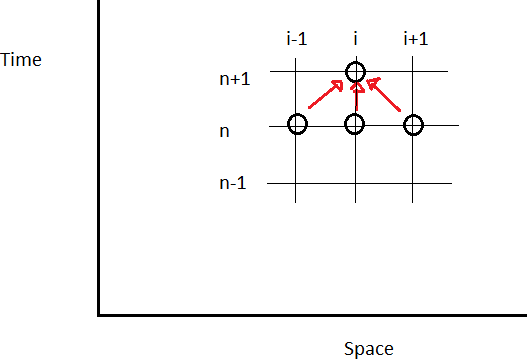
\includegraphics[scale=0.4]{report/stencil.png}\\
The basic technique of multi-processors programming is splitting the tasks between multiples processors meaning that the result matrix is going to be split. But how ? it could be horizontally, vertically and in cube where every processor is in charge of one part of the matrix, see picture below.\\

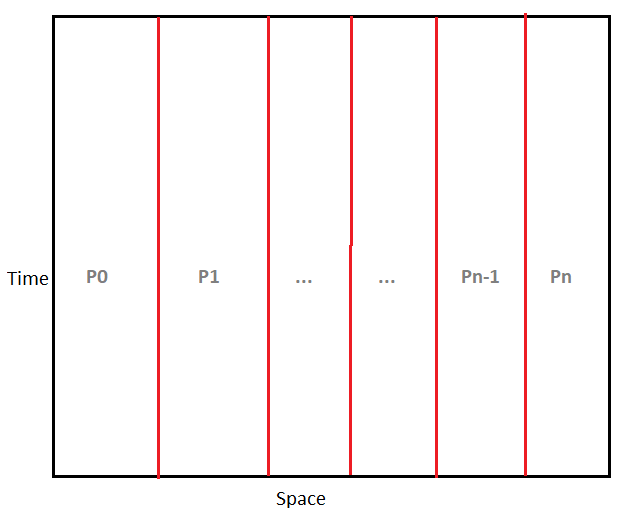
\includegraphics[scale=0.3]{report/vertical.png} 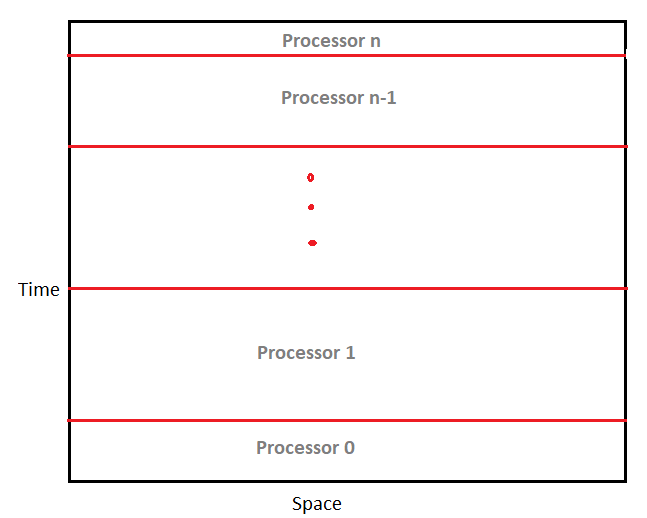
\includegraphics[scale=0.3]{report/horizontal.png}\\ 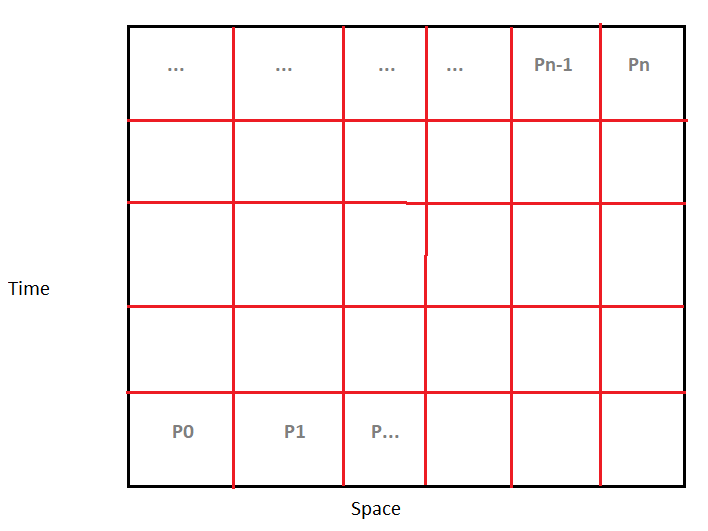
\includegraphics[scale=0.4]{report/cube.png} \\
To chose a way of dividing the matrix, we need to take a look of the dependencies between the different point in time and space, the stencil.
Looking at the equation stencil, it is clear that if we split the matrix horizontally ( meaning each matrix would take care of a time step and every space step ) the performance would not increase because for one processor to compute it would have to wait for the previous processor to finish its job. Making the program serial because only one processor would be working at a time.\\
So we will be splitting the matrix vertically. It implies that when reaching a "boundary", the processor has to receive and send a result to its neighbor processor.\\
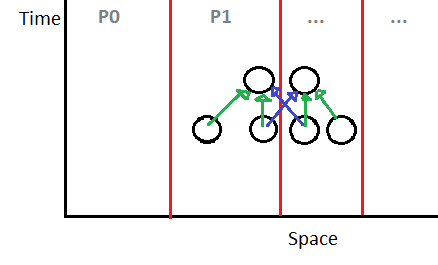
\includegraphics[scale=0.5]{report/stencilVertical.png}\\
The above picture represents how the work is divided in this particular case, the green arrow are value that does not need to be transferred because the processor already has the correct value meanwhile the blue arrows represents value that are transmitted from one processor to another.
\section{Results}
	As discuss earlier, there is a dilemma between the gain of processing time and the inferred communication costs. The more processor you have, the smallest the sub matrices are but the more communication there is.\\
	Every problem has its own balance, let's see how this apply in this case with a 21*100 matrix ( $\Delta x$=0.05 and $\Delta t$=0.01).
\subsection{Numerical value}
	The result from the parallel program are the same as the one with the serial program which is a good thing, because some precision can be lost during the communication. Here is the plot of the value for $t=0.5$.\\
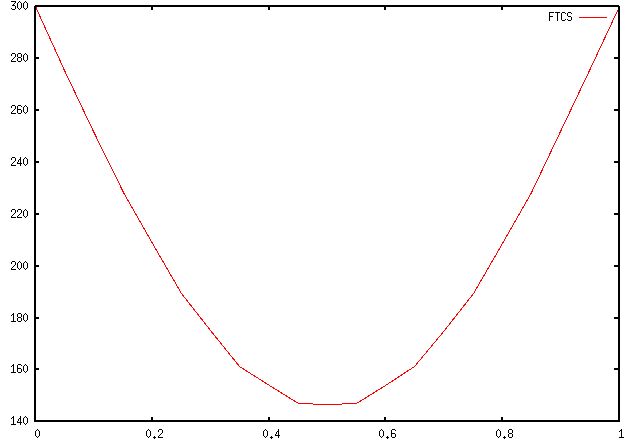
\includegraphics[scale=0.5]{report/FTCS}
\subsection{Time performance}
We can assume that the time for the serial program and the time for the parallel program with one processor is the same. After verification, it is. The time is 0.1 ms on average of 10 tries.


\end{document}